\subsection{Neurones}\label{chapter-ML-section-DNN-neuron}
\subsubsection{Principe}
Un neurone est une entité ayant
un certain nombre d'entrées $x_i$, $i\in\set{1,\ldots,n}$,
auxquelles sont associées des poids $w_i$,
un biais $b$
et
une fonction $f$ dite d'\og activation \fg, discutée section~\ref{chapter-ML-section-DNN-neuron-activ_fct}.
Les poids $w_i$ et le biais $b$ sont les paramètres du neurone,
la fonction d'activation est un hyper-paramètre.
La sortie $s$ du neurone s'exprime
\begin{equation}
s = f\left(\sum_{i=1}^n w_ix_i + b\right)
\mend
\end{equation}
Le fonctionnement d'un neurone est résumé sur la figure~\ref{fig-chapter-ML-section-DNN-neuron-neuron_structure}.
\begin{figure}[h]
\centering
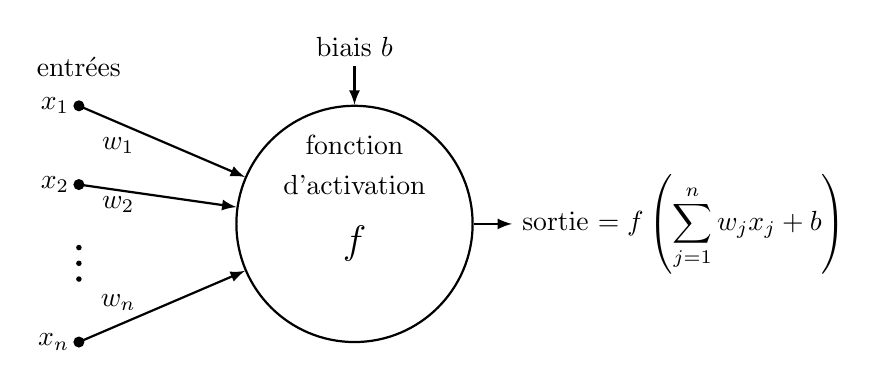
\begin{tikzpicture}

\node [draw, thick, circle, minimum size = 3 cm] (N) at (0,0) {};

\foreach \yi/\N in {1.5/1,0.5/2,-1.5/n}{
\fill (-3.5,\yi) circle(2pt) node [left] {$x_{\N}$};
\draw [thick, -latex] (-3.5,\yi) -- (N);
}

\draw (-3.5,1.75) node [above] {entrées};

\draw (-3,1) node {$w_1$};
\draw (-3,0.25) node {$w_2$};
\draw (-3,-1) node {$w_n$};

\foreach \x/\y in {-3.5/-.5}{
\fill (\x,\y) circle (1pt);
\fill (\x,\y+.2) circle (1pt);
\fill (\x,\y-.2) circle (1pt);
}

\draw [thick, latex-] (N) -- (0,2) node [above] {biais $b$};

\draw [thick, -latex] (N) -- (2,0) node (output) [right] {sortie $\displaystyle = f\left(\sum_{j=1}^n w_jx_j + b\right)$};

\draw (0,-.25) node {\Large $f$};
\draw (0,1) node {fonction};
\draw (0,.5) node {d'activation};

\end{tikzpicture}

\caption[Structure d'un neurone.]{Structure d'un neurone. Une fonction $f$ dite d'\og activation \fg{} est appliquée à la somme des entrées $x_i$ pondérées par les poids $w_i$ et du biais $b$ afin d'obtenir la valeur de sortie.}
\label{fig-chapter-ML-section-DNN-neuron-neuron_structure}
\end{figure}
\subsubsection{Fonctions d'activation}\label{chapter-ML-section-DNN-neuron-activ_fct}
En principe, toute fonction définie sur l'ensemble d'existence des entrées $x_i$ peut être utilisée comme fonction d'activation.
Celles-ci étant généralement à valeurs réelles et unidimensionnelles, les fonctions sont définies sur $\mathbb{R}$.
Les plus utilisées sont:
\begin{description}
\item[tangente hyperbolique] notée $\tanh$, définie par
\begin{equation}
\tanh(x) = \frac{\eexp{x}-\eexp{-x}}{\eexp{x}+\eexp{-x}}
\label{eq-act_fct-tanh}
\mend[;]
\end{equation}
\item[sigmoïde] notée $\mathrm{sig}$, définie par
\begin{equation}
\mathrm{sig}(x) = \frac{\eexp{x}}{1+\eexp{x}} = \frac{1}{1+\eexp{-x}}
\label{eq-act_fct-sig}
\mend[;]
\end{equation}
\item[Softsign] notée $\mathrm{Ssg}$, définie par
\begin{equation}
\mathrm{Ssg}(x) = \frac{x}{1+\abs{x}}
\label{eq-act_fct-ssg}
\mend[;]
\end{equation}
\item[ReLU] (\emph{Rectified Linear Unit}), définie par
\begin{equation}
\mathrm{ReLU}(x)
=
\left\lbrace \begin{aligned}
x\msep & x > 0\\
0 & x \leq 0
\end{aligned} \right.
\label{eq-act_fct-relu}
\mend[;]
\end{equation}
\item[Softplus] notée $\mathrm{Spl}$, définie par
\begin{equation}
\mathrm{Spl}(x)
=
\ln(1+\eexp{x})
\label{eq-act_fct-spl}
\mend[;]
\end{equation}
\item[ELU] (\emph{Exponential Linear Unit}), définie par
\begin{equation}
\mathrm{ELU}(x)
=
\left\lbrace \begin{aligned}
x\msep & x > 0\\
\alpha(\eexp{x}-1)\msep & x \leq 0
\end{aligned} \right.
\msep
\alpha=1
\label{eq-act_fct-elu}
\mend[;]
\end{equation}
\item[SELU] (\emph{Scaled Exponential Linear Unit}), définie par
\begin{equation}
\mathrm{SELU}(x)
=
\lambda\times\left\lbrace \begin{aligned}
x\msep & x > 0\\
\alpha(\eexp{x}-1)\msep & x \leq 0
\end{aligned} \right.
\msep
\alpha \simeq \num{1.67}
\msep
\lambda \simeq \num{1.05}
\label{eq-act_fct-selu}
\mend[;]
\end{equation}
\end{description}

\todo{figure with plots for some activation functions}